%!TEX root = ../report.tex

\begin{document}
    \chapter{附加功能}

	
	\section{键鼠交互的相机旋转移动}
	\subsection{平移旋转变换}
	\begin{spacing}{2.5}
	其实,所谓相机的旋转移动可以看成相机固定不动,而物体在进行逆变换,例如,相机左移一个单位其实就是物体向右移动一个单位。因此要相机的旋转移动,只要实现物体对应的旋转移动即可。所用到的变换矩阵如下:
	\begin{enumerate}
		\item 平移变换矩阵
		\begin{equation}
		\begin{pmatrix}
			1 &  0&  0&0 \\ 
 			0&  1&  0& 0\\ 
 			0& 0 & 1 &0 \\ 
 			T_{x}&  T_{y}&  T_{z}& 1
		\end{pmatrix}
		\label{transfer_1}
		\end{equation}
		\item 	绕X轴旋转变换矩阵
		\begin{equation}
		\begin{pmatrix}
			 1&  0&  0 &0 \\ 
 			0&  cos\theta &  sin\theta& 0\\ 
 			 0& -sin\theta & cos\theta &0 \\ 
 			0&  0&  0& 1
		\end{pmatrix}
		\label{yrotate}
		\end{equation}
		\item 绕Y轴旋转变换矩阵
		\begin{equation}
		\begin{pmatrix}
			cos\theta &  0&  -sin\theta &0 \\ 
 			0&  1&  0& 0\\ 
 			sin\theta & 0 & cos\theta &0 \\ 
 			0&  0&  0& 1
		\end{pmatrix}
		\label{xrotate}	
		\end{equation}
	
		\item 绕Z轴旋转变换矩阵
		\begin{equation}
		\begin{pmatrix}
			cos\theta &  sin\theta &  0 &0 \\ 
 			-sin\theta &  cos\theta &  0& 0\\ 
 			0 & 0 & 1 &0 \\ 
 			0&  0&  0& 1
		\end{pmatrix}
		\label{zrotate}
		\end{equation}
		\item 缩放变换矩阵
		\begin{equation}
		\begin{pmatrix}
			S_{x}& 0 &  0 &0 \\ 
 			0 &  S_{y} &  0& 0\\ 
 			0 & 0 & S_{z} &0 \\ 
 			0&  0&  0& 1
		\end{pmatrix}
		\label{zrotate}
		\end{equation}
	\end{enumerate}
	\end{spacing}

	\subsection{键鼠交互}
\begin{spacing}{2.5}
		为了增加交互性,我们自己加入了键鼠交互方面的功能,即:键盘通过上下左右或WASD键可以进行视角的移动、通过TAB可以切换场景,鼠标通过拖动也可以实现视角的移动,这些移动本质上是通过物体坐标的改变来实现的\\
	首先需要一个全局事件监听函数,响应event并判断对应的类型,最后执行特定功能函数:
\end{spacing}

	\begin{lstlisting}
void App::OnEvent(SDL_Event* event , double dt)
{
	switch (event->type)
	{
		case SDL_QUIT:
			running = false;
			break;

        case SDL_MOUSEBUTTONDOWN:
            mouseIsDown = 1;
            break;

        case SDL_MOUSEBUTTONUP:
            mouseIsDown = 0;
            break;
        
        case SDL_MOUSEMOTION:
            if(mouseIsDown){
                onMouseDrag(*event);
                break;
            }
            break;

		case SDL_KEYDOWN:
            onKeyPress(event->key.keysym.sym , dt);
            break;
        
		default:
			break;
	}
}
	\end{lstlisting}
	\begin{spacing}{2.5}
			键盘的监听可以使用SDL2库中的键盘事件接口来实现:
	\end{spacing}

\begin{lstlisting}
void App::onKeyPress(SDL_Keycode keyCode , double dt) {
    auto camera = Camera::getInstance();
    auto v = 45;
    auto velo = camera->getMoveVelo();
    switch (keyCode) {
        case SDLK_ESCAPE:
            running = false;
            break;
        case SDLK_w:
            camera->offsetPosition(camera->forward() * velo * dt);
            break;
        case SDLK_s:
            camera->offsetPosition(-camera->forward() * velo * dt);
            break;
        case SDLK_a:
            camera->offsetPosition(-camera->right() * velo * dt);
            break;
        case SDLK_d:
            camera->offsetPosition(camera->right() * velo * dt);
            break;
        case SDLK_z:
            camera->offsetPosition(camera->up() * velo * dt);
            break;
        case SDLK_x:
            camera->offsetPosition(-camera->up() * velo * dt);
            break;
        case SDLK_UP:
            camera->offsetDirection(v * dt, 0);
            break;
        case SDLK_DOWN:
            camera->offsetDirection(-v * dt, 0);
            break;
        case SDLK_LEFT:
            camera->offsetDirection(0, -v*dt);
            break;
        case SDLK_RIGHT:
            camera->offsetDirection(0, v *dt);
            break;
        case SDLK_TAB:
            Camera::getInstance()->resetCamera();
            Canvas::getInstance()->addScene();
            Canvas::getInstance()->resetNode();
            break;
        default:
            break;
    }
}
\end{lstlisting}

	\begin{spacing}{2.5}
			鼠标的监听则要复杂一些,因为要实现拖动的交互效果,SDL2中并没有直接的接口,需要先通过MouseIsDown进行判断,如果鼠标被按下,则调用MouseMotion监听鼠标移动轨迹,通过方向、速率等参数传达到移动函数中,最后调整一些参数,使得拖动效果看起来更真实
	\end{spacing}

\begin{lstlisting}
void App::onMouseDrag(SDL_Event& event) {
    auto v = 45;
    auto camera = Camera::getInstance();
    auto velo = camera->getMoveVelo();
    camera->offsetPosition(camera->right() * velo * event.motion.xrel * 0.001);
    camera->offsetPosition(-camera->up() * velo * event.motion.yrel * 0.001);
    camera->offsetDirection(0 , -v * event.motion.xrel * 0.0028);
    camera->offsetDirection( v * event.motion.yrel * 0.0028, 0);
}
\end{lstlisting}

    \section{区域填充}
    \begin{spacing}{2.5}
    本渲染器用到的区域填充算法是课堂中学过的扫描线填充算法,不同的是这里分了更多情况进行优化分析,在通常情况下,扫描线填充算法运用于一般多边形是比较复杂的,所以项目中我们都采取先转化为三角形单元的形式,但是三角形也分为一般三角形、平底三角形和平顶三角形,后面两种三角形对于扫描线算法而言非常友好,因为其一边可以恰好与扫描线重合。
    对于一般三角形,可以采取从中间分成一个平底三角形和平顶三角形的策略来进行扫描,最后扫描的情况只需要分别针对这两种特殊的三角形即可:
	    \begin{figure}[H]
		\centering
		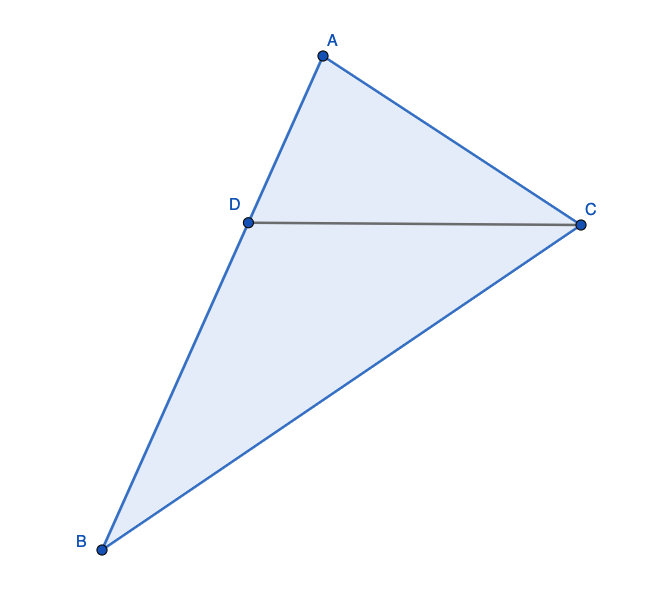
\includegraphics[width=0.6\textwidth]{images/scanline1.png}
		\caption{普通三角形的切分}
		\label{line}
	\end{figure}
	
比如上图的普通三角形ABC,就可以分为一个平底三角形ACD和一个平顶三角形BCD

    \end{spacing}
        \begin{lstlisting}
    if (MathUtil::equal(pVert1->pos.y, pVert2->pos.y)) 
    {
        triangleBottomRasterize(*pVert1, *pVert2, *pVert3);
    }
    else if (MathUtil::equal(pVert2->pos.y, pVert3->pos.y))
    {
        triangleTopRasterize(*pVert1, *pVert2, *pVert3);
    }
    else
    {
        double ty = pVert2->pos.y;
        double factor = (ty - pVert1->pos.y) / (pVert3->pos.y - pVert1->pos.y);
        VertexOut tVert = pVert1->interpolate(*pVert3, factor);
        triangleTopRasterize(*pVert1, tVert, *pVert2);
        triangleBottomRasterize(*pVert2, tVert, *pVert3);
    }

        \end{lstlisting}

    \begin{spacing}{2.5}
    对于平顶三角形而言,扫描线于顶部重合,自顶向下循环遍历y值,通过比例计算插值从而计算出中间情况的需要填充的像素,scanLineFill直接调用底层的drawPixel对像素进行着色
    
    	
    \end{spacing}

	\begin{lstlisting}
    for (int py = startPY; py * sign <= sign * endPY; py = py + sign)
    {
    	double ld = 1.0f;
       	double factor = (py - startPY) * ld / (endPY - startPY);
       	VertexOut vertStart = pVert1->interpolate(*pVert2, factor);
       	VertexOut vertEnd = pVert1->interpolate(*pVert3, factor);
       	scanLineFill(vertStart, vertEnd, py);
   	}
	\end{lstlisting}


    \section{纹理贴图}
    
    \section{光照}
    
    \section{三维模型}
    
    \section{天空盒子}
\end{document}
